\documentclass[11pt]{article}
\usepackage[paperwidth=24cm, paperheight=50cm, margin=2cm]{geometry}
\usepackage{tikz}
\usetikzlibrary{shapes.geometric, arrows.meta, positioning, fit, calc}

\begin{document}

\begin{center}
\textbf{\huge Johansen Cointegration Test -- Code Flowchart} \\[1em]
\textit{\large Execution flow of johansen.py (Dark Wing Financial Mathematics)}
\end{center}

\vspace{1cm}

\begin{center}
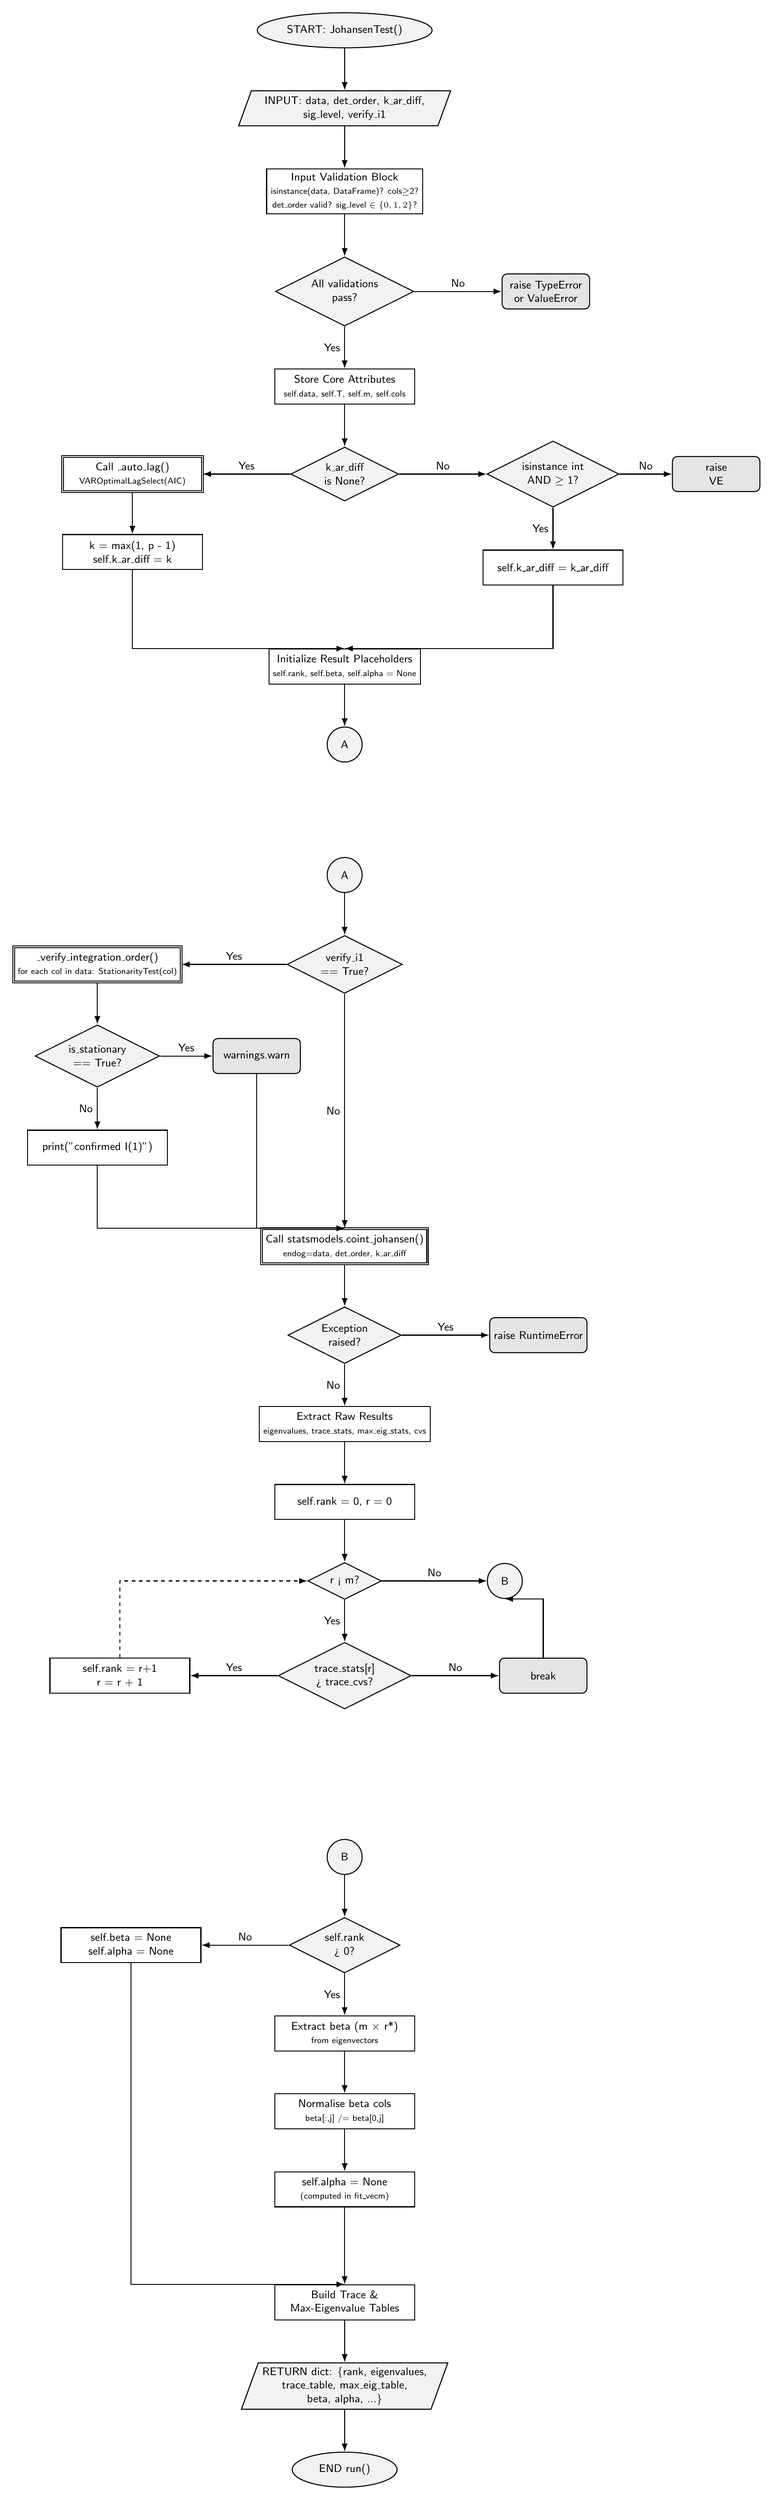
\begin{tikzpicture}[
  >=Latex,
  node distance=1.2cm and 1.5cm,
  font=\sffamily\small,
  term/.style={ellipse, draw, thick, minimum width=3cm, minimum height=1cm, align=center, fill=black!5},
  io/.style={trapezium, trapezium left angle=70, trapezium right angle=-70, draw, thick, minimum width=3cm, minimum height=1cm, align=center, fill=black!5},
  proc/.style={rectangle, draw, thick, minimum width=4cm, minimum height=1cm, align=center, fill=white},
  dec/.style={diamond, draw, thick, aspect=2, align=center, fill=black!5},
  sub/.style={rectangle, draw, thick, double, minimum width=4cm, minimum height=1cm, align=center, fill=white},
  err/.style={rectangle, draw, thick, rounded corners, minimum width=2.5cm, minimum height=1cm, align=center, fill=black!10},
  conn/.style={circle, draw, thick, minimum width=1cm, align=center, fill=black!5}
]

% -------------------------------------------------------------------------
% SECTION 1: __init__
% -------------------------------------------------------------------------
\node [term] (start) {START: JohansenTest()};
\node [io, below=of start] (inputs) {INPUT: data, det\_order, k\_ar\_diff,\\ sig\_level, verify\_i1};
\node [proc, below=of inputs] (val) {Input Validation Block\\ \scriptsize{isinstance(data, DataFrame)? cols$\ge$2?}\\ \scriptsize{det\_order valid? sig\_level $\in \{0,1,2\}$?}};
\node [dec, below=of val] (val_ok) {All validations\\ pass?};
\node [err, right=of val_ok, xshift=1cm] (raise_val) {raise TypeError\\ or ValueError};
\draw [->, thick] (val_ok) -- node[above] {No} (raise_val);

\node [proc, below=of val_ok] (store) {Store Core Attributes\\ \scriptsize{self.data, self.T, self.m, self.cols}};
\draw [->, thick] (start) -- (inputs);
\draw [->, thick] (inputs) -- (val);
\draw [->, thick] (val) -- (val_ok);
\draw [->, thick] (val_ok) -- node[left] {Yes} (store);

\node [dec, below=of store] (k_none) {k\_ar\_diff\\ is None?};
\draw [->, thick] (store) -- (k_none);

\node [sub, left=of k_none, xshift=-1cm] (auto_lag) {Call \_auto\_lag()\\ \scriptsize{VAROptimalLagSelect(AIC)}};
\node [proc, below=of auto_lag] (k_calc) {k = max(1, p - 1)\\ self.k\_ar\_diff = k};
\draw [->, thick] (k_none) -- node[above] {Yes} (auto_lag);
\draw [->, thick] (auto_lag) -- (k_calc);

\node [dec, right=of k_none, xshift=1cm] (k_int) {isinstance int\\ AND $\ge$ 1?};
\node [err, right=of k_int] (raise_k) {raise\\ VE};
\node [proc, below=of k_int] (k_store) {self.k\_ar\_diff = k\_ar\_diff};
\draw [->, thick] (k_none) -- node[above] {No} (k_int);
\draw [->, thick] (k_int) -- node[above] {No} (raise_k);
\draw [->, thick] (k_int) -- node[left] {Yes} (k_store);

\node [proc, below=of k_none, yshift=-3cm] (init_place) {Initialize Result Placeholders\\ \scriptsize{self.rank, self.beta, self.alpha = None}};
\draw [->, thick] (k_calc.south) |- (init_place.north);
\draw [->, thick] (k_store.south) |- (init_place.north);

\node [conn, below=of init_place] (conn_A) {A};
\draw [->, thick] (init_place) -- (conn_A);

% -------------------------------------------------------------------------
% SECTION 2: run()
% -------------------------------------------------------------------------
\node [conn, below=of conn_A, yshift=-1.5cm] (conn_A_in) {A};
\node [dec, below=of conn_A_in] (verify_i1) {verify\_i1\\ == True?};
\draw [->, thick] (conn_A_in) -- (verify_i1);

\node [sub, left=of verify_i1, xshift=-1.5cm] (stat_test) {\_verify\_integration\_order()\\ \scriptsize{for each col in data: StationarityTest(col)}};
\node [dec, below=of stat_test] (is_stat) {is\_stationary\\ == True?};
\node [err, right=of is_stat] (warn) {warnings.warn};
\node [proc, below=of is_stat] (conf) {print("confirmed I(1)")};

\draw [->, thick] (verify_i1) -- node[above] {Yes} (stat_test);
\draw [->, thick] (stat_test) -- (is_stat);
\draw [->, thick] (is_stat) -- node[above] {Yes} (warn);
\draw [->, thick] (is_stat) -- node[left] {No} (conf);

\node [sub, below=of verify_i1, yshift=-5.5cm] (call_johansen) {Call statsmodels.coint\_johansen()\\ \scriptsize{endog=data, det\_order, k\_ar\_diff}};
\draw [->, thick] (conf.south) |- (call_johansen.north);
\draw [->, thick] (warn.south) |- (call_johansen.north);
\draw [->, thick] (verify_i1) -- node[left] {No} (call_johansen);

\node [dec, below=of call_johansen] (exc) {Exception\\ raised?};
\node [err, right=of exc, xshift=1cm] (raise_run) {raise RuntimeError};
\draw [->, thick] (call_johansen) -- (exc);
\draw [->, thick] (exc) -- node[above] {Yes} (raise_run);

\node [proc, below=of exc] (extract) {Extract Raw Results\\ \scriptsize{eigenvalues, trace\_stats, max\_eig\_stats, cvs}};
\draw [->, thick] (exc) -- node[left] {No} (extract);

\node [proc, below=of extract] (init_r) {self.rank = 0, r = 0};
\draw [->, thick] (extract) -- (init_r);

\node [dec, below=of init_r] (loop_r) {r < m?};
\node [conn, right=of loop_r, xshift=1.5cm] (conn_B) {B};
\draw [->, thick] (init_r) -- (loop_r);
\draw [->, thick] (loop_r) -- node[above] {No} (conn_B);

\node [dec, below=of loop_r] (trace_gt) {trace\_stats[r]\\ > trace\_cvs?};
\draw [->, thick] (loop_r) -- node[left] {Yes} (trace_gt);

\node [proc, left=of trace_gt, xshift=-1cm] (rank_plus) {self.rank = r+1\\ r = r + 1};
\node [err, right=of trace_gt, xshift=1cm] (break_loop) {break};
\draw [->, thick] (trace_gt) -- node[above] {Yes} (rank_plus);
\draw [->, thick] (trace_gt) -- node[above] {No} (break_loop);

\draw [->, thick, dashed] (rank_plus.north) |- (loop_r.west);
\draw [->, thick] (break_loop.north) |- (conn_B.south);

% -------------------------------------------------------------------------
% SECTION 3 & 4: extract beta and return
% -------------------------------------------------------------------------
\node [conn, below=of trace_gt, yshift=-2.5cm] (conn_B_in) {B};
\node [dec, below=of conn_B_in] (rank_gt_0) {self.rank\\ > 0?};
\draw [->, thick] (conn_B_in) -- (rank_gt_0);

\node [proc, left=of rank_gt_0, xshift=-1cm] (beta_none) {self.beta = None\\ self.alpha = None};
\node [proc, below=of rank_gt_0] (extract_beta) {Extract beta (m $\times$ r*)\\ \scriptsize{from eigenvectors}};
\node [proc, below=of extract_beta] (norm_beta) {Normalise beta cols\\ \scriptsize{beta[:,j] /= beta[0,j]}};
\node [proc, below=of norm_beta] (alpha_none) {self.alpha = None\\ \scriptsize{(computed in fit\_vecm)}};

\draw [->, thick] (rank_gt_0) -- node[above] {No} (beta_none);
\draw [->, thick] (rank_gt_0) -- node[left] {Yes} (extract_beta);
\draw [->, thick] (extract_beta) -- (norm_beta);
\draw [->, thick] (norm_beta) -- (alpha_none);

\node [proc, below=of alpha_none, yshift=-1cm] (build_tabs) {Build Trace \&\\ Max-Eigenvalue Tables};
\draw [->, thick] (alpha_none) -- (build_tabs);
\draw [->, thick] (beta_none.south) |- (build_tabs.north);

\node [io, below=of build_tabs] (ret_dict) {RETURN dict: \{rank, eigenvalues,\\ trace\_table, max\_eig\_table,\\ beta, alpha, ...\}};
\draw [->, thick] (build_tabs) -- (ret_dict);

\node [term, below=of ret_dict] (end_run) {END run()};
\draw [->, thick] (ret_dict) -- (end_run);

\end{tikzpicture}
\end{center}

\vspace{2cm}

\begin{center}
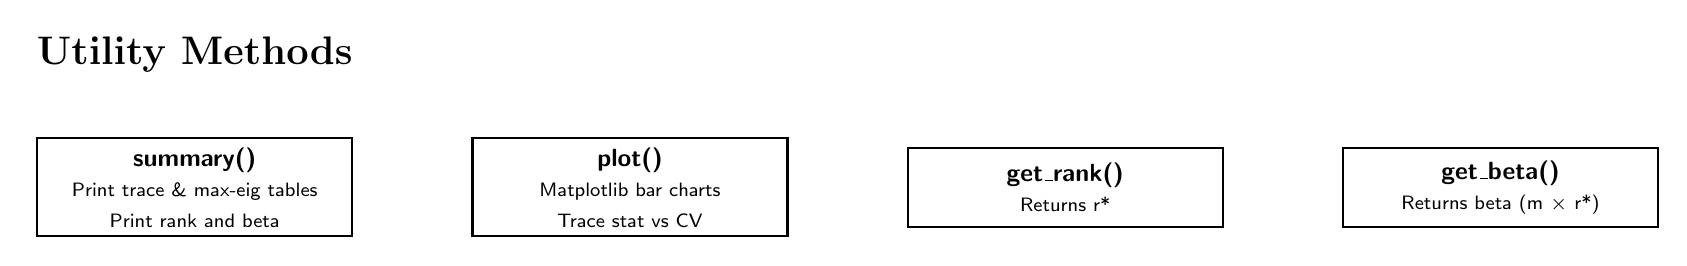
\begin{tikzpicture}[
  >=Latex,
  node distance=1.2cm and 1.5cm,
  font=\sffamily\small,
  proc/.style={rectangle, draw, thick, minimum width=4cm, minimum height=1cm, align=center, fill=white}
]
% -------------------------------------------------------------------------
% SECTION 5: UTILITY METHODS
% -------------------------------------------------------------------------
\node[font=\Large\bfseries] (util_title) {Utility Methods};
\node[proc, below=of util_title, yshift=0.5cm] (summary) {\textbf{summary()}\\ \scriptsize{Print trace \& max-eig tables}\\ \scriptsize{Print rank and beta}};
\node[proc, right=of summary] (plot) {\textbf{plot()}\\ \scriptsize{Matplotlib bar charts}\\ \scriptsize{Trace stat vs CV}};
\node[proc, right=of plot] (get_rank) {\textbf{get\_rank()}\\ \scriptsize{Returns r*}};
\node[proc, right=of get_rank] (get_beta) {\textbf{get\_beta()}\\ \scriptsize{Returns beta (m $\times$ r*)}};
\end{tikzpicture}
\end{center}

\end{document}
